\subsection{Measured heat loads in the LHC}
\label{seq:measured}

It is known from measurements at the LHC, that the total heat loads for most cryogenic cells do not fall below 0.8$\cdot10^{-13}$ W/hc/p+ (Watts per half cell and proton) even after long periods of scrubbing.
This includes the expected contribution of impedance and direct synchrotron radiation heating (see. Fig.~\ref{fig:measured_hl}).

In the scope of this report, especially the low heat load cells are of interest.
Figure~\ref{fig:special} shows the heat loads in the special instrumented cells during a typical fill in early 2017.
It becomes clear that at high energy, the majority of the heat load is measured at the dipoles.
During the ramp, the contribution of the quadrupoles is strongly decreasing.
Most of the drift space should also be part of the "quadrupole" contribution in these plots.

\begin{figure}[tbh]
    \centering
    \includegraphics[width=0.8\textwidth]{../plots/004_plot_0_All_cells_at_stop_squeeze_1.png}
    \caption{An overview of the occurring heat loads in the LHC from 2015 to early 2017.}
    \label{fig:measured_hl}
\end{figure}

\begin{figure}[tbh]
    \centering
    \includegraphics[width=0.8\textwidth]{../ss/027_spec_5885_Special_instrumented_cells_for_fill_5885_1.png}
    \caption{The heat load of the special instrumented cell for a typical fill in early 2017.
    Each cell contains several temperature sensors before and after the 3 dipole magnets (D2, D3, D4) and the quadrupole/Short Straight Section (Q1).}
    \label{fig:special}
\end{figure}



\clearpage

\subsection{Heat loads from simulations}
To estimate the effect of photoelectrons on the buildup simulations, a simulation study that includes the common magnets in a cryogenic cell of the LHC is presented here.
Each of these magnets is simulated either with photoemission seeding or with an initial distribution of electrons.
The normally used magnetic fields for a beam with an energy of 6.5~TeV are shown in the following table, its content has been extracted either from MADX files or from the settings of the LHC control system for a standard physics fill in 2016.
Their lengths have been inferred from MADX input files for the LHC.
\begin{center}
    \begin{tabular}{llll}
        \textbf{Magnet} & \textbf{Length} [m]&\textbf{B} & \textbf{B\_skew}\\ \hline
        Drift & 5.79 & - & - \\
        Main Bend & 42.90 & 7.73 T& - \\
        Horizontal corrector magnet & 0.32 & 2.72 T & - \\
        Vertical corrector magnet & 0.32 & - & 2.32 T \\
        Main quadrupole & 3.46 & 174.78 T/m& - \\
        Main sextupole ($+$)& 0.35 & 758.86 T/m$^2$ & - \\
        Main sextupole ($-$) & 0.35 & -1300.9 T/m$^2$ & - \\
        Main octupole & 0.15 & 57817.78 T/m$^3$ & - \\
    \end{tabular}
\end{center}

Figure~\ref{fig:simulation} shows the heat loads per meter for a two trains of 288 bunches, consisting of 4 batches of 72 bunches, with a bunch intensity of 1.1$\cdot10^{11}$ p/bunch.
The batches are interleaved with 8 empty bunch slots, and the trains with 30 slots.
The heat load from the second train has been rescaled to 2512 bunches, in order to arrive at a heat load that corresponds to a filled LHC machine with 2800 bunches in total, without having to simulate each bunch.
This procedure is valid since the electron-cloud in the trains starting from the second are identical in case the electron density is saturated by the end of the first train.
The right axes correspond to the heat load scaled to the length each element has in a typical cryogenic cell of the LHC arcs.

So far, only simulations with the conservative estimates for the photoemission parameters have been performed for most elements, with the exception of the drifts.
It is clear that dipoles, quadrupoles and drift spaces are most the most relevant devices in terms of total heat load, since they are far longer than the higher order and correction magnets.
Another conclusion is that the photoemission seeding only has a significant impact on drifts and dipoles.

Figure~\ref{fig:summed_hl} shows the summed up heat loads, with the same SEY for all devices.
This is assumed to be a reasonable choice, since after several years of operation, the surfaces of the LHC beam screen which are exposed to the electron cloud should all be scrubbed to the maximum effect.
In addition, the expected contributions from the resistive wall effect and the absorption of synchrotron radiation are indicated.
The vertical dashed line states a lower limit in normalized heat load, as derived from Fig.~\ref{fig:measured_hl}.

Figure~\ref{fig:simulation2} shows the impact that some modifications to simulation process have on the resulting heat loads, while Fig.~\ref{fig:simulation_electrons} features the electron densities for drift simulations.
These modifications include:
\begin{itemize}
    \item the distribution of new macroparticles from initially reflected photons, see Sec.~\ref{sec:photon_cdf}.
        This change is not visible in the results at all.
    \item a generation of photoelectrons that is constant in time (continuous), see Sec.~\ref{sec:delay}.
        The only effect is an higher electron density in between bunches, however the heat loads are unchanged.
    \item a correct 3D cosine distribution of the initial velocity of new MPs, relative to the surface normal (Sec.~\ref{sec:cosine3D}).
        This has a very large effect on all devices, but note that also the generation of MPs from secondary emission has been changed.
        Most likely, this effect is responsible for the large changes in heat loads and electron densities.
\end{itemize}

\begin{figure}[tbh]
    \centering
    \begin{minipage}[c]{0.8\textwidth}
        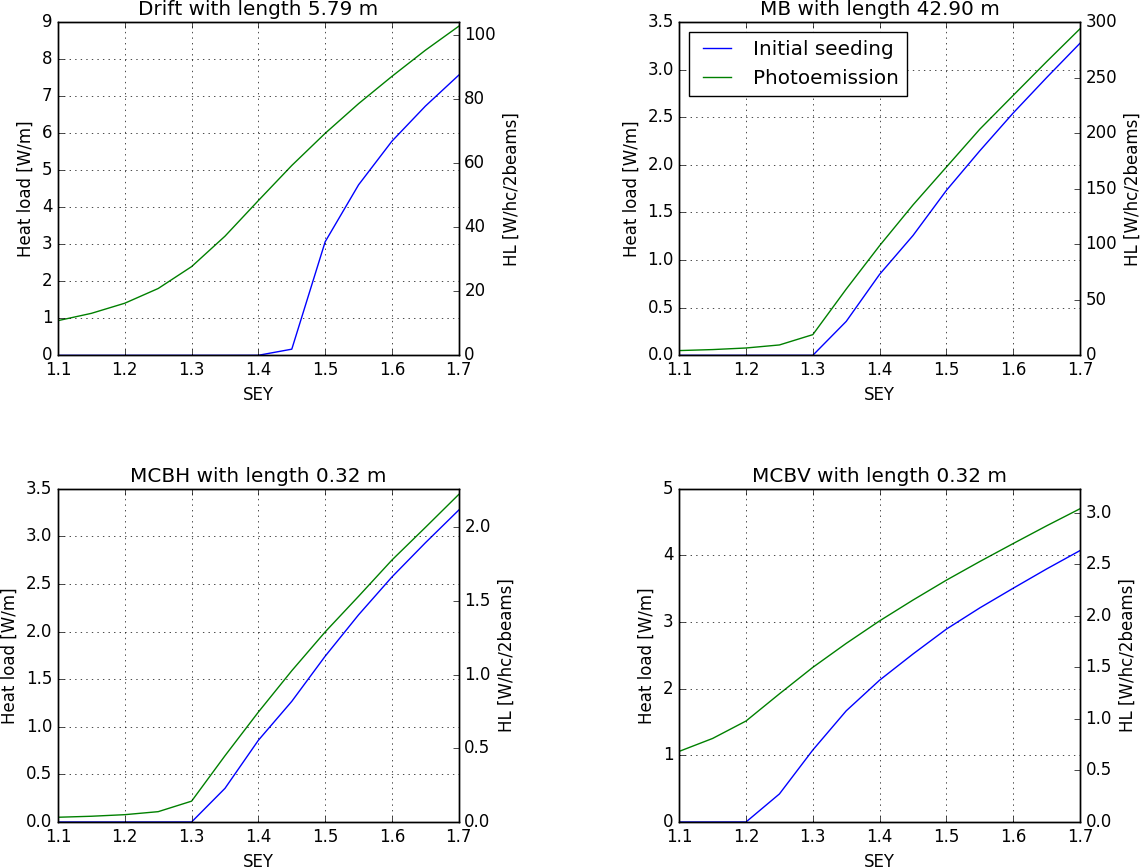
\includegraphics[width=\textwidth]{../plots/study_2.png}
    \end{minipage}

    \vspace{0.5cm}

    \begin{minipage}[c]{0.8\textwidth}
        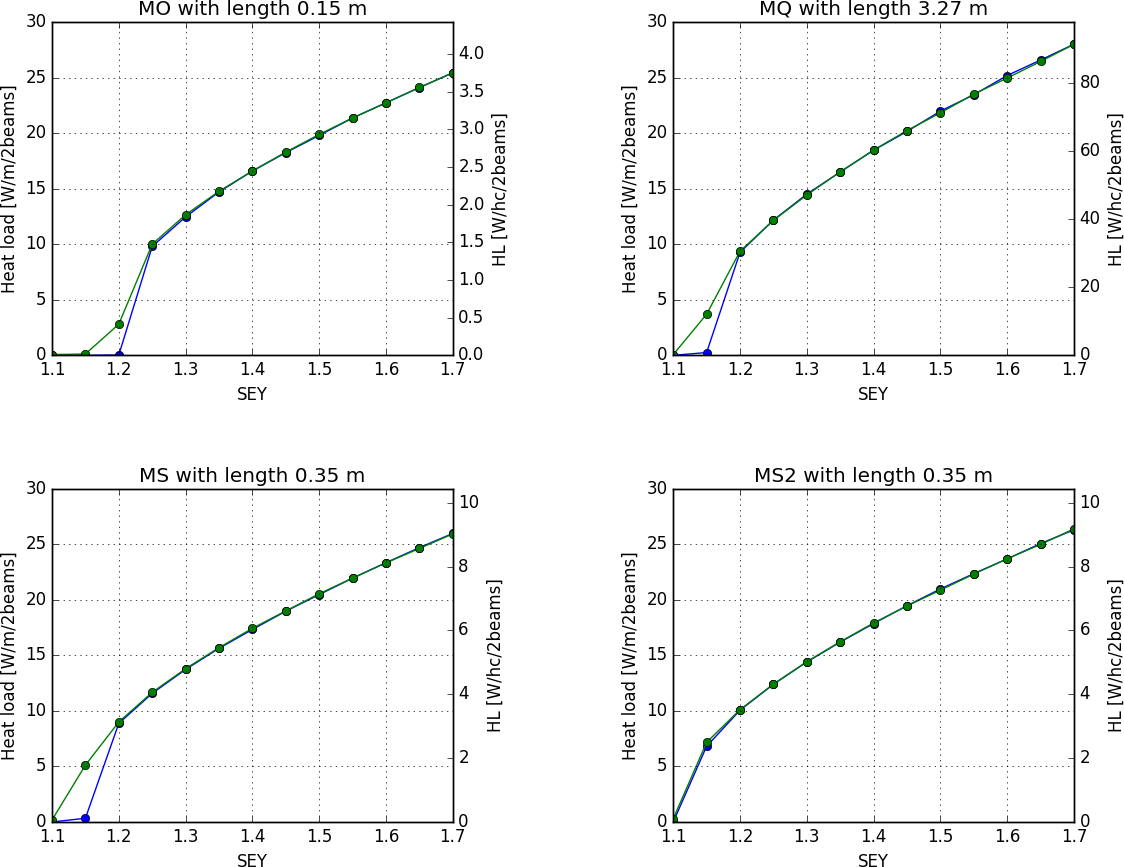
\includegraphics[width=\textwidth]{../plots/study_3.png}
    \end{minipage}
    \caption{These are the resulting heat loads from simulations with "conservative" photoemission parameters derived in Sec.~\ref{sec:best} and magnetic field parameters from Sec.~\ref{sec:simulation}.
    In case of the drifts, also the "realistic" parameters have been simulated.}
    \label{fig:simulation}
\end{figure}


\begin{figure}[tbh]
    \centering
    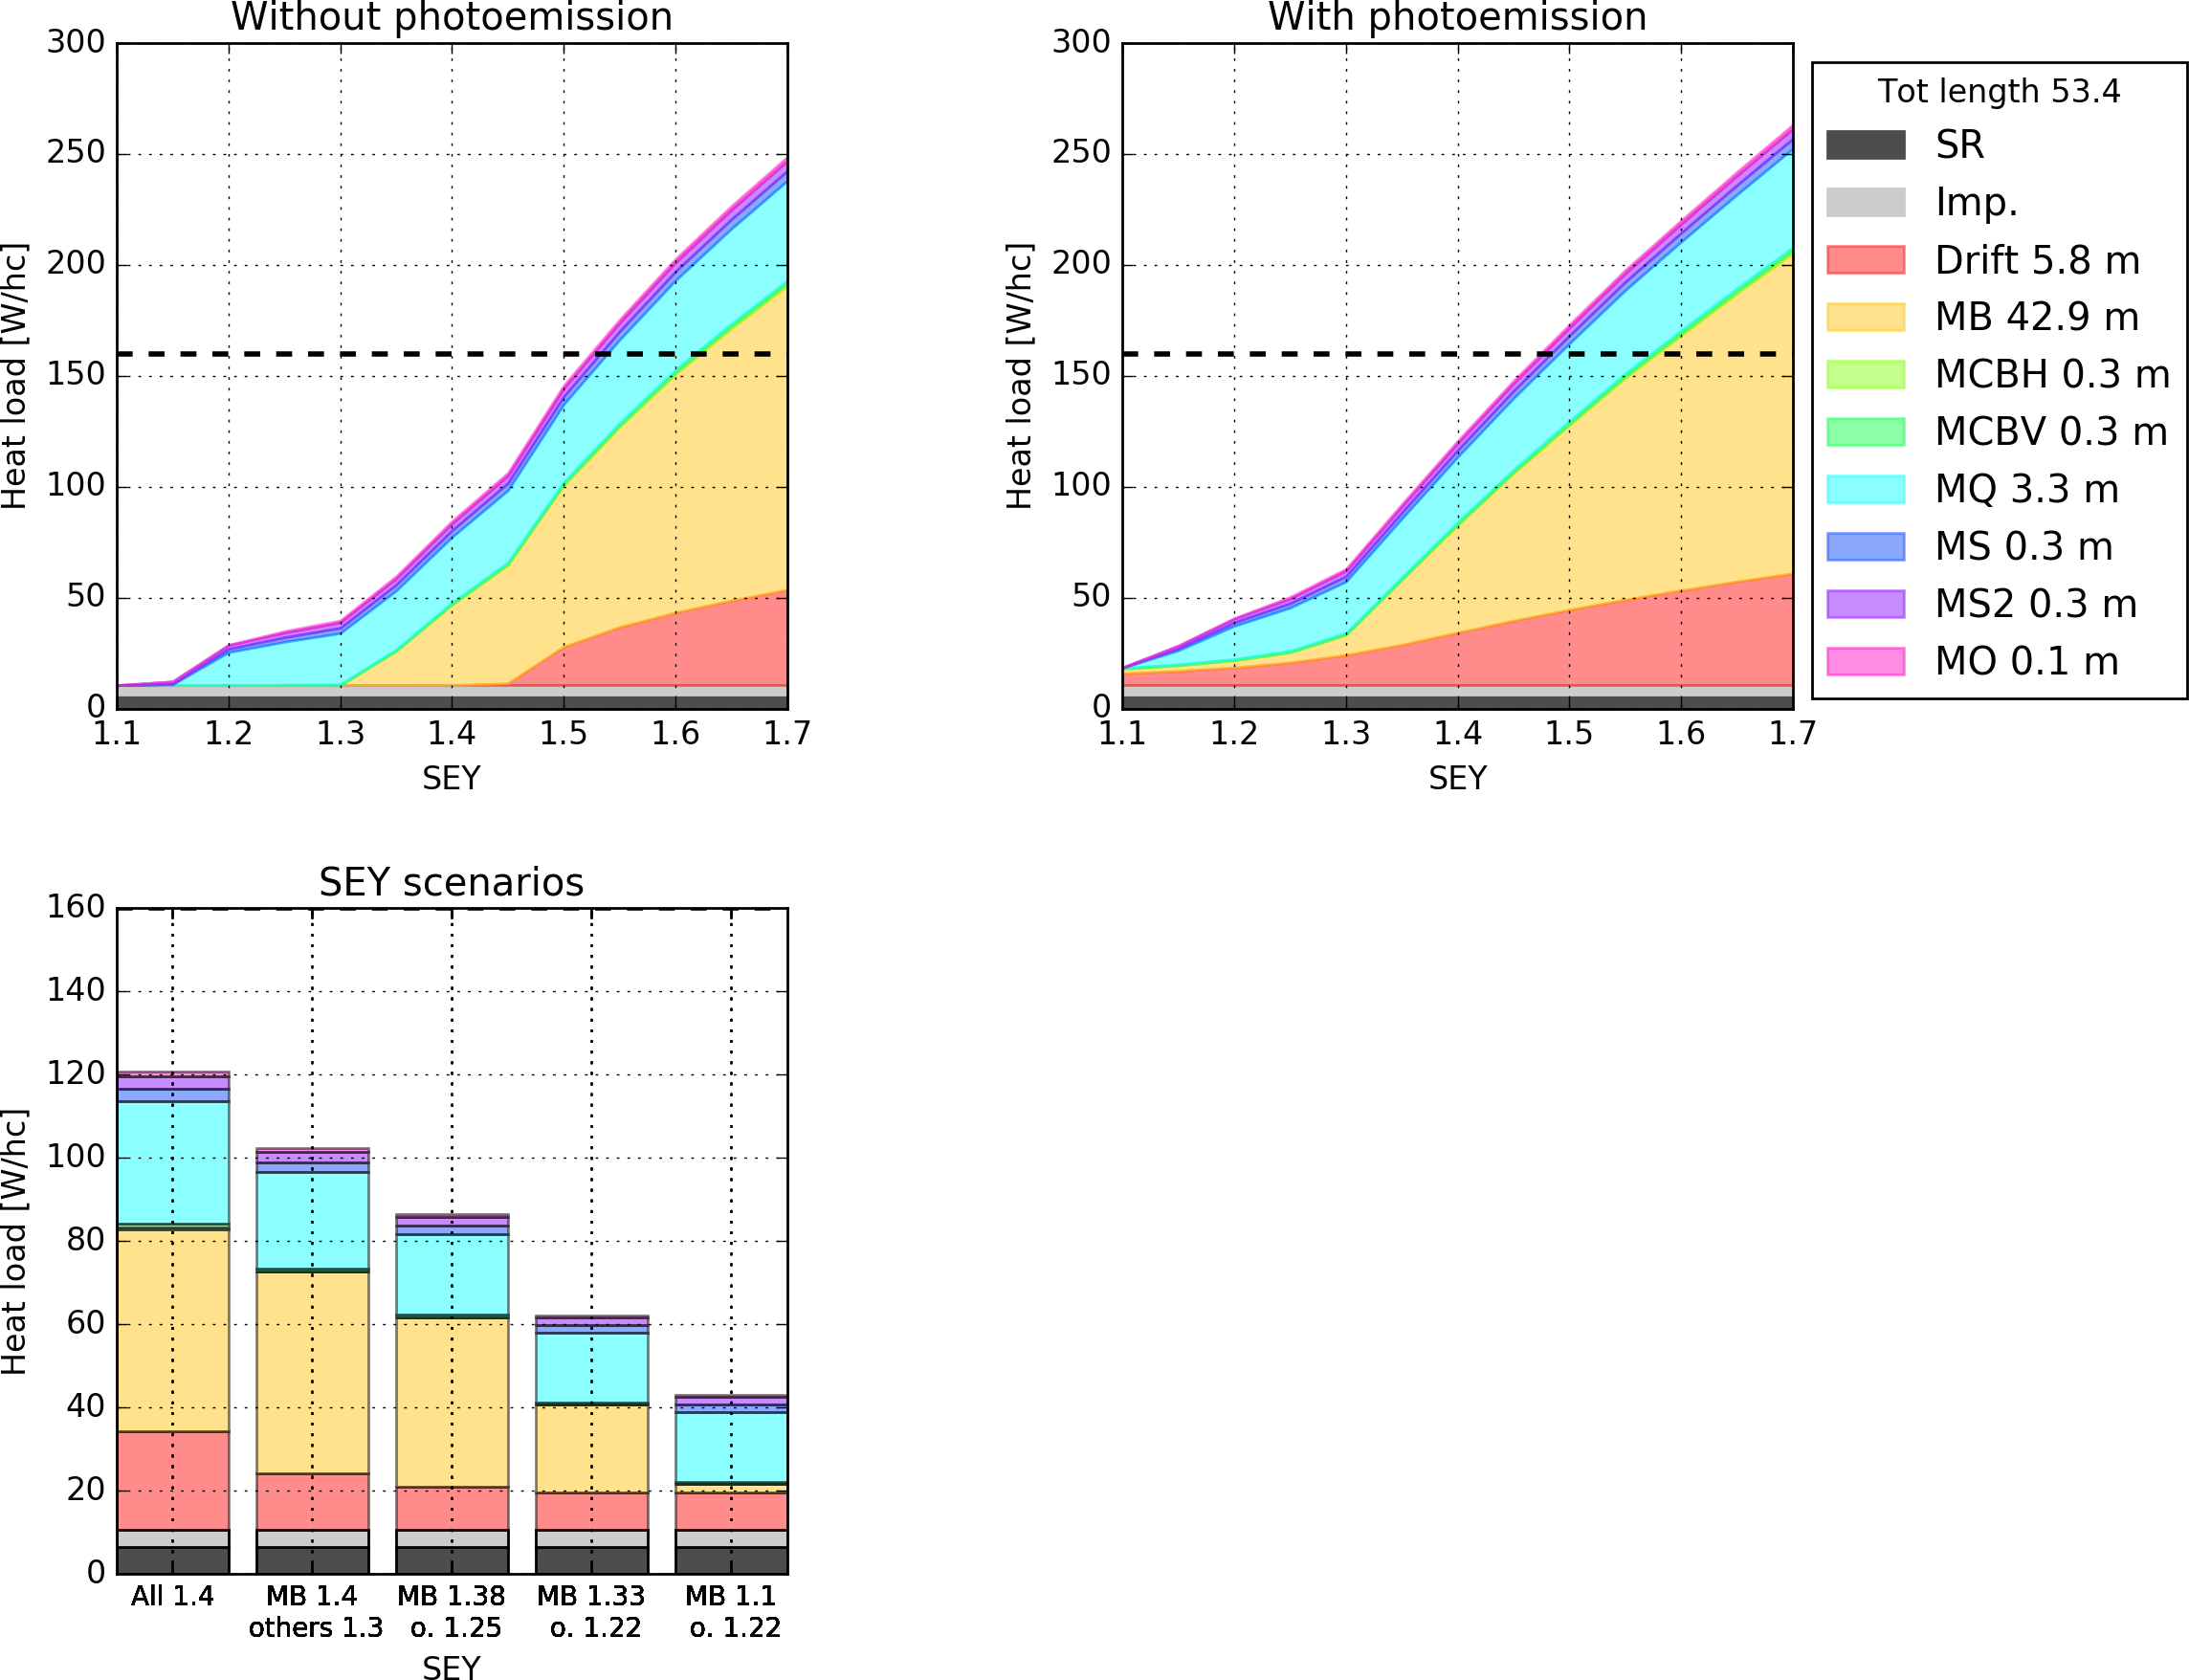
\includegraphics[width=0.9\textwidth]{../plots/summed_hl_1.png}
    \caption{The top two plots add up the heat loads for the same value of the SEY, which gives a rough overview about the relative impact of each element.
    The bottom plot shows the cumulative heat loads for different combinations of SEY values.
    }
    \label{fig:summed_hl}
\end{figure}

\begin{figure}[tbh]
    \centering
    \begin{minipage}[c]{0.8\textwidth}
        \includegraphics[width=\textwidth]{../plots/study_4.png}
    \end{minipage}

    \vspace{0.5cm}

    \begin{minipage}[c]{0.8\textwidth}
        \includegraphics[width=\textwidth]{../plots/study_5.png}
    \end{minipage}
    \caption{
        The different simulations with variants of photoemission parameters are compared here.
        They include the angular distribution of newly generated macroparticles, and the distribution of photoelectrons from reflected photons.
        Additionally, also a constant rate of photoemission has been simulated.
    }
    \label{fig:simulation2}
\end{figure}

\begin{figure}[tbh]
    \centering
    \includegraphics[width=0.8\textwidth]{../plots/study_6.png}
    \caption{The electrons in the chamber during simulations of a drift at an SEY parameter of 1.5 are shown here.
    In the left plot, the amount of new photoelectrons is varied.
    In the right plot, modifications to the simulations were made.}
    \label{fig:simulation_electrons}
\end{figure}

\subsection{Comparison of measured and simulated heat loads}

When comparing the measured heat loads from Fig.~\ref{fig:measured_hl} and the simulation results from Fig.~\ref{fig:summed_hl}, there seems to be a very good agreement of the lowest heat load cells and simulations of a very low SEY parameter in case photoemission seeding is activated.
The normalized heat loads in both cases are compatible.
However if also the information from the special cells (Fig.~\ref{fig:special} is taken into account, it becomes clear that the measured heat loads at high energy are mostly measured in the dipoles, whereas the simulated heat loads at a low SEY parameter are dominated by the drift spaces, due to the contribution of photoelectrons.



